\documentclass[11pt,a4paper]{article}

\usepackage[margin=2.5cm]{geometry}
\usepackage{amsmath}
\usepackage{amssymb}
\usepackage{booktabs}
\usepackage{longtable}
\usepackage{array}
\usepackage{ragged2e}
\usepackage{seqsplit}
\usepackage{enumitem}
\usepackage{xcolor}
\usepackage{listings}
\usepackage[hidelinks]{hyperref}
\usepackage{caption}

%--------------------------
%  GRAPHICS / FIGURES
%--------------------------
\usepackage{float}
\usepackage{graphicx}

\DeclareGraphicsExtensions{.pdf}
\graphicspath{{figs/}}


% \file wraps long paths/identifiers at any character rather than running
% into the margin; inline use renders the same as plain \texttt.
\newcommand{\file}[1]{\texttt{\seqsplit{#1}}}
\newcommand{\code}[1]{\texttt{#1}}
\newcommand{\Rinf}{\ensuremath{R_\infty}}
\newcommand{\Rwhite}{\ensuremath{R_{\mathrm{white}}}}
\newcommand{\srcref}[1]{\par\smallskip{\footnotesize\itshape\RaggedRight #1\par}}
\setlength{\emergencystretch}{3em}
\newcolumntype{L}[1]{>{\RaggedRight\arraybackslash}p{#1}}

% Code listing style: line numbers on the left are set with firstnumber to the
% real line number in the source file, so a number in the margin is the number
% you will find the line at today.
\definecolor{codebg}{gray}{0.96}
\lstdefinestyle{py}{
  language=Python,
  basicstyle=\ttfamily\footnotesize,
  backgroundcolor=\color{codebg},
  frame=single,
  numbers=left,
  numberstyle=\tiny\color{gray},
  breaklines=true,
  breakatwhitespace=true,
  showstringspaces=false,
  keywordstyle=\color{blue!55!black},
  commentstyle=\color{green!35!black},
  stringstyle=\color{red!45!black},
  captionpos=b,
}

\title{\Rinf: the paper-referenced reflectance\\
\large What it is, how to read it, how it is computed, and where it is used}
\author{Colorimeter project --- pad analysis pipeline}
\date{Generated 2026-09-07 against branch \file{preimage-capture}}

\begin{document}
\maketitle

\begin{abstract}
\noindent
\Rinf{} is the per-pixel, per-cell reflectance of the indicator pad
\emph{re-referred to the strip's own bare paper}.  It is the fourth link in
the photometric chain \code{sig} $\to$ \code{R} $\to$ \Rinf{} $\to$
\code{A}\,/\,\code{K/S}, and it is the quantity \code{contact\_sheet(\ldots,
quantity="R\_inf")} draws and \code{cell\_table} tabulates by default.  This
note collects its definition, its interpretation, the equations and the
actual code that computes it, and every place it is consumed downstream.
\end{abstract}

\tableofcontents
\newpage

%======================================================================
\section{What \Rinf{} is}
%======================================================================

\subsection{One sentence}

\Rinf{} is a dimensionless number, one per pad pixel and per
\emph{cell}\footnote{A \emph{cell} is one (LED,~Bayer-layer) pair --- the
project's unit of spectral measurement, e.g.\ \code{royal\_blue.B}.  Exposure
is not part of it.}, equal to the pad's reflectance against the two gray
chips divided by that same reflectance measured on the strip's own unstained
paper.  On the bare paper itself it is $1$ by construction; on a stained pad
it drops below~$1$ in the bands the dye absorbs.

\subsection{Where it sits in the chain}

The pad-analysis pipeline turns sensor counts into a dose-proportional
quantity in six steps, each a separate pure function in
\file{desktop/padanalysis/padphot.py} so that each can be read and checked on
its own.\footnote{\file{desktop/padanalysis/padphot.py}, module docstring,
lines 8--16.  Reproduced verbatim below.}

\begin{lstlisting}[style=py,firstnumber=8,caption={\texttt{padphot.py} module docstring --- the chain.}]
    sig   = lit - dark                    counts, done by probe.Capture.layer
    div   = divisor(...)                  the gray-chip level at this region
    R     = reflectance(sig, div)         referred to the gray chips
    R_inf = reflectance_infinity(R, Rw)   referred to a diffuse white
    A     = absorbance(R_inf)             -log10(R)
    f     = km_remission(R_inf)           (1-R)^2 / 2R  =  K/S
    dKS   = delta_ks(f, f_blank)          the dose-proportional quantity
\end{lstlisting}

\paragraph{``Against''.}
Throughout, ``\code{R} against the gray chips'' and ``\Rinf{} against the
bare paper'' use \emph{against} to mean \emph{referenced to} --- that is,
\emph{divided by the reference value taken from}.  Both \code{R} and \Rinf{}
are ratios of one signal to another; ``against~X'' names the denominator.

\code{R} is reflectance against the gray chips: \code{R = 1} means ``as
bright as the chips''.  The chips are a working reference, not a calibrated
diffuse white, and they belong to the stage rather than to the strip, so a
change of gray card between sessions moves every \code{R}.  \Rinf{} removes
that by dividing \code{R} through by the strip's own paper, which was
photographed in the same frame, under the same illuminant, with no
chemistry on it: \Rinf{} = 1 then means ``as bright as the bare paper''.

The chip reference is a \emph{single number} for the whole pad
(equation~\eqref{eq:div}).  \file{desktop/padanalysis/R\_inf\_guide.py}
draws every step and weighs that one number against a per-pixel alternative;
its conclusion is that for \Rinf{} the choice cannot matter, because the
divisor cancels (see the remark under equation~\eqref{eq:Rinf}).

\subsection{Why ``infinity''}

The name follows Kubelka--Munk.  \Rinf{} in that theory is the reflectance
of an \emph{optically thick} layer --- one deep enough that no light reaches
the backing.  The remission function
\begin{equation}
  f(\Rinf) = \frac{(1-\Rinf)^2}{2\Rinf} = \frac{K}{S}
  \label{eq:km}
\end{equation}
is linear in absorber concentration only for such a layer, and only when
\Rinf{} is measured against a stable diffuse white --- assumption~(iv) of
\file{tex/gutzeit\_analysis.tex}, \S``Reflectance photometry''.\footnote{%
\file{tex/gutzeit\_analysis.tex}, \S\,Reflectance photometry, lines
894--931; equation \eqref{eq:km} is \code{eq:km} at lines 903--908,
assumption (iv) is at line 920.}  The function name
\code{reflectance\_infinity} is the code asserting that this is the quantity
being produced; whether the pad really is optically thick is a separate
question the pipeline does not settle.

%======================================================================
\section{How to interpret \Rinf{}}
%======================================================================

\begin{description}[style=nextline,leftmargin=1.4cm]

\item[$\Rinf \approx 1$ on the bare paper.]
This is exact by construction and is the pipeline's arithmetic self-check.
Running \code{cell\_table("C1020", roi=ROIWHITE)} must give \code{R\_inf} =
$1.0000$, \code{A} $\approx 0$ and \code{K/S} $\approx 0$ for every cell.  If
any of those drifts, the chain is mis-wired and nothing downstream is
trustworthy.\footnote{\file{desktop/padanalysis/HOWTO.md}, \S\,8.4 ``The
arithmetic check'', lines 453--467.}

\item[$\Rinf < 1$: the pad is darker than its own paper.]
Dye is present in this band.  The deeper below~$1$, the more the pad absorbs
at that wavelength.  A heavily stained pad in the blue cells runs well
below~$1$.

\item[$\Rinf > 1$: the pad is brighter than its paper.]
Expected in the red and amber cells, where no arsenic product absorbs and
the pad body can scatter slightly more than the reference patch of paper.
Also what photometric noise does on a blank pad, straddling $\Rinf = 1$.
Because $f(R)$ has its minimum at $R=1$ and rises on \emph{both} sides, a
pad reading a little above~$1$ gets a positive $K/S$ indistinguishable from
one a little below; average $K/S$ over such a region with
\code{km\_remission\_signed} (attribute \code{KS\_signed}), not
\code{km\_remission}.\footnote{\file{desktop/padanalysis/padphot.py},
\code{km\_remission}, lines 220--266 (the ``Trap'' paragraph);
\code{km\_remission\_signed}, lines 269--297.}

\item[Spectral shape.]
Read across the cells in wavelength order, \Rinf{} on the pad should climb
monotonically through the absorption edge: on C1020, roughly
\code{violet.B}~$0.66 \to$ \code{royal\_blue.B}~$0.77 \to$
\code{blue}~$0.88 \to$ \code{cyan}~$0.93 \to$ \code{green}~$0.99 \to$
\code{amber}/\code{red} slightly above~$1.0$.  A non-monotone spectrum is a
bad cell, not chemistry.\footnote{\file{desktop/padanalysis/HOWTO.md}, \S\,8.4,
lines 464--467.}

\item[\Rinf{} is not dose-proportional by itself.]
It still carries the pad's scattering and the session.  Only the blank-%
subtracted remission $\Delta(K/S) = f(\Rinf)_{\text{exposed}} -
f(\Rinf)_{\text{blank}}$ is approximately proportional to arsenic loading
(equation \code{eq:dks} of the tex).  The blank is the strip's own
pre-image where it has one.

\item[The reference can be missing.]
The bare paper is about twice as bright as the gray chips, so on the short
wavelengths it reaches the sensor ceiling one or two exposure rungs before
the pad does.  When the paper clipped, \Rwhite{} and everything past it
(\Rinf, \code{A}, \code{K/S}) are \code{None}; the pad's \code{R} is still
valid.  \code{BalancedCell.paper\_clipped} says so and \code{cell\_table}
prints the row rather than dropping it.\footnote{%
\file{desktop/padanalysis/analysis\_1.py}, \code{BalancedCell} docstring,
lines 883--897; the guard is at lines 1036--1038.}

\item[The choice of white does not divide out.]
$f(R)$ is non-linear, so referring \code{R} to the gray chips and referring
it to the paper give genuinely different $K/S$, and the difference is not a
constant factor.  This is why \code{reflectance\_infinity} demands the
reference as an explicit argument and has no default.\footnote{%
\file{desktop/padanalysis/padphot.py}, module docstring, lines 28--32.}

\end{description}

%======================================================================
\section{How \Rinf{} is used}
%======================================================================

\begin{description}[style=nextline,leftmargin=1.4cm]

\item[\code{contact\_sheet(samp\_no, quantity="R\_inf")}]
Draws every modelled cell of one sweep as a small image panel on one shared
scale (\Rinf{} spans $0$ to $1.4$), so a dead pixel, a dropped layer or a
stray reflection is visible, and the pad's colour shows as the pad going
dark in the blue cells and not the red.\footnote{%
\file{desktop/padanalysis/analysis\_1.py}, \code{contact\_sheet}, lines
1376--1442; the \Rinf{} display range is set at line 1407.}

\item[\code{cell\_table(samp\_no, quantity="R\_inf")}]
\Rinf{} is the \emph{default} \code{quantity}.  Prints one row per cell ---
$n$, mean, std, and the 10th/50th/90th percentiles --- the numeric companion
to the contact sheet, and the tool used for the arithmetic check on
\code{ROIWHITE}.\footnote{\file{desktop/padanalysis/analysis\_1.py},
\code{cell\_table}, signature and default at lines 1445--1446.}

\item[\code{pre\_post\_overlay(samp\_no, LED, Bayerlayer)}]
Divides the measurement's \Rinf{} by the registered pre-image's \Rinf{}
pixel by pixel.  Structure in that ratio that follows the pad outline is a
registration error; structure inside the pad is chemistry.\footnote{%
\file{desktop/padanalysis/analysis\_1.py}, \code{pre\_post\_overlay}, lines
1499--1583; the ratio is formed at line 1559.}

\item[The downstream transforms.]
\code{absorbance(R\_inf)}, \code{km\_remission(R\_inf)} and
\code{km\_remission\_signed(R\_inf)} all take \Rinf{} as input; \code{A},
\code{KS} and \code{KS\_signed} on a \code{BalancedCell} are computed from it
and are \code{None} exactly when it is.

\item[The driver menu.]
\code{run\_sampno} steps 4--6 select \code{"R\_inf"} as the quantity to plot
or list.\footnote{\file{desktop/padanalysis/analysis\_1.py},
\code{run\_sampno}, lines 1775--1805.}

\end{description}

%======================================================================
\section{How \Rinf{} is computed}
%======================================================================

\subsection{The equations}

For one cell, one exposure rung, over the pixels of one region:
\begin{align}
  \mathrm{div}
    &= w_1\,\langle \mathrm{sig}\rangle_{\text{chip1}}
     + w_2\,\langle \mathrm{sig}\rangle_{\text{chip2}}
     &&\text{gray-chip level at this region}
     \label{eq:div}\\[2pt]
  R  &= \frac{\mathrm{sig}}{\mathrm{div}}
     &&\text{reflectance against the chips}
     \label{eq:R}\\[2pt]
  \Rwhite &= \operatorname*{median}_{p\,\in\,\text{paper}} R_p
     &&\text{scalar white reference}
     \label{eq:Rw}\\[4pt]
  \boxed{\;\Rinf = \dfrac{R}{\Rwhite}\;}
     &&&\text{paper-referenced reflectance}
     \label{eq:Rinf}\\[4pt]
  A &= -\log_{10}\Rinf, \qquad
  f(\Rinf) = \frac{(1-\Rinf)^2}{2\,\Rinf}
     &&\text{the two linearising transforms}
     \nonumber
\end{align}

Here $\langle\cdot\rangle_{\text{chip}}$ is the mean of the dark-subtracted
signal over a gray-chip mask, and $w_1, w_2$ are the two interpolation
weights from the cell's fitted flat-field surface
(\file{whitecorr.anchor\_weights}), recomputed for the region actually being
measured because the illumination is not flat between the chips.

Two details of \eqref{eq:Rw} that the equation hides:
\begin{itemize}[nosep]
  \item \Rwhite{} is taken in the \emph{same sweep} the cell came from ---
        a pre-image is referred to its own paper, a measurement to its own.
  \item the code recomputes reflectance from the raw, unregistered
        full-frame signal for the paper median rather than reusing the
        \code{R} array, because \code{R} is masked to the requested region
        (which need not overlap the paper) and, for a pre-image, has been
        resampled onto the measurement grid.
\end{itemize}

\paragraph{The divisor cancels.}
\code{div} is a single number, so it divides out of \eqref{eq:Rinf}
entirely:
\[
  \Rinf
  = \frac{\mathrm{sig}_{\text{pad}} / \mathrm{div}}
         {\operatorname{median}(\mathrm{sig}_{\text{paper}}) / \mathrm{div}}
  = \frac{\mathrm{sig}_{\text{pad}}}
         {\operatorname{median}(\mathrm{sig}_{\text{paper}})}.
\]
So the \emph{value} of \code{div} --- and the flat-field surface behind its
weights --- never reaches \Rinf, \code{A} or \code{K/S}.  It reaches only
\code{R} (equation~\eqref{eq:R}) and anything built from \code{R} before the
paper step, such as \file{duotone.PadCube}.  Replacing the one number with a
per-pixel divisor \emph{would} change \Rinf, because it takes different
values over the pad and over the paper and so no longer cancels; whether
that is an improvement is a question about the flat-field model, worked
through in \file{desktop/padanalysis/R\_inf\_guide.py}.

\subsection{The code: the pure transforms}

Each of the three steps is one line of arithmetic plus a positivity guard.

\begin{lstlisting}[style=py,firstnumber=95,caption={\texttt{padphot.py} --- \code{divisor()}, equation \eqref{eq:div}.}]
    w1, w2, *_ = anchor_weights(model, region, chip1, chip2)
    return w1 * float(np.mean(sig[chip1])) + w2 * float(np.mean(sig[chip2]))
\end{lstlisting}
\srcref{\file{desktop/padanalysis/padphot.py}, function \code{divisor},
lines 61--96 (body shown: 95--96).}

\begin{lstlisting}[style=py,firstnumber=131,caption={\texttt{padphot.py} --- \code{reflectance()}, equation \eqref{eq:R}.}]
    if not div > 0:
        raise ValueError(f"divisor must be positive, got {div!r}")
    return sig / div
\end{lstlisting}
\srcref{\file{desktop/padanalysis/padphot.py}, function \code{reflectance},
lines 101--133 (body shown: 131--133).}

\begin{lstlisting}[style=py,firstnumber=180,caption={\texttt{padphot.py} --- \code{reflectance\_infinity()}, equation \eqref{eq:Rinf}.}]
    if np.any(np.asarray(R_white) <= 0):
        raise ValueError("R_white must be positive")
    return R / R_white
\end{lstlisting}
\srcref{\file{desktop/padanalysis/padphot.py}, function
\code{reflectance\_infinity}, lines 136--182 (body shown: 180--182).  The
parameter is named \code{R\_white}; the returned value is \Rinf.}

\begin{lstlisting}[style=py,firstnumber=215,caption={\texttt{padphot.py} --- the two transforms that consume \Rinf.}]
    # absorbance(R), l. 187-215
    return -np.log10(np.maximum(R, MIN_REFLECTANCE))
    # km_remission(R_inf), l. 220-266
    r = np.maximum(R_inf, MIN_REFLECTANCE)
    return (1.0 - r) ** 2 / (2.0 * r)
\end{lstlisting}
\srcref{\file{desktop/padanalysis/padphot.py}: \file{absorbance} lines
187--215; \file{km\_remission} lines 220--266; \file{km\_remission\_signed}
lines 269--297.  \file{MIN\_REFLECTANCE}~$=10^{-6}$ keeps $-\log_{10}$ and
the denominator finite on a dead pixel.}

\subsection{The code: where the steps are assembled}

\code{get\_balanced\_cell\_data} reads one cell, picks its exposure rung,
builds the region masks, and walks the chain, storing every intermediate on
a \code{BalancedCell}.

\begin{lstlisting}[style=py,firstnumber=1016,caption={\texttt{analysis\_1.py} --- \code{get\_balanced\_cell\_data()}, the assembly of \Rinf.}]
    raw_sig, raw_lit = got

    # References are read in the sweep the cell came from, on the whole
    # frame, before any registration: the chips do not move with the strip.
    chip1 = _region(samp_no, ROIGRAY1, sec)
    chip2 = _region(samp_no, ROIGRAY2, sec)
    paper = _region(samp_no, ROIWHITE, sec, erode)
    measured = _region(samp_no, roi, sec, erode)

    div = padphot.divisor(model, measured, chip1, chip2, raw_sig)

    a = get_cell_data(samp_no, LED, Bayerlayer, roi=roi, sec=sec,
                      erode=erode, rung=rung, register=register)
    if a is None:
        return None
    R = padphot.reflectance(a, div)

    # The paper's own saturation screen.  It clips before the pad does on
    # the short wavelengths, and when it has, this cell simply has no
    # per-strip white reference at this rung -- R stays valid.
    paper_sat = float((raw_lit[paper] >= SATURATED_DN).mean())
    if paper_sat > MAX_SAT_FRACTION:
        R_white = R_inf = A = KS = KS_signed = None
    else:
        R_white = float(np.median(padphot.reflectance(raw_sig, div)[paper]))
        R_inf = padphot.reflectance_infinity(R, R_white)
        A = padphot.absorbance(R_inf)
        KS = padphot.km_remission(R_inf)
        KS_signed = padphot.km_remission_signed(R_inf)
\end{lstlisting}
\srcref{\file{desktop/padanalysis/analysis\_1.py}, function
\code{get\_balanced\_cell\_data}, lines 919--1057; block shown: 1016--1044.
\Rinf{} is computed at line 1041.}

\begin{lstlisting}[style=py,firstnumber=900,caption={\texttt{analysis\_1.py} --- \code{BalancedCell} keeps \Rinf{} and reports its mean.}]
    __slots__ = ("samp_no", "cell", "roi", "sec", "rung", "exposure_us",
                 "sig", "div", "R", "R_white", "R_inf", "A", "KS",
                 "KS_signed", "sat_frac", "paper_sat", "paper_clipped")
    ...
        return (head + f" R_inf={self.R_inf.mean():.4f}"
                f" A={self.A.mean():+.4f} KS={self.KS_signed.mean():+.5f}>")
\end{lstlisting}
\srcref{\file{desktop/padanalysis/analysis\_1.py}, class \code{BalancedCell},
lines 872--916; \code{\_\_slots\_\_} at 900--902, attribute documentation at
883--891, \code{\_\_repr\_\_} \Rinf{} at line 915.}

%======================================================================
\section{Where \Rinf{} appears in the code}
%======================================================================

Every occurrence, grouped by file.  Line numbers are as of the generation
date above.

\subsection*{\file{desktop/padanalysis/padphot.py} --- the definitions}

\begin{description}[style=nextline,leftmargin=1.2cm,font=\normalfont]
\item[module docstring, l.\,8--16]
  names \Rinf{} as step~4 of the chain,
  \code{R\_inf = reflectance\_infinity(R, Rw)}.
\item[\code{reflectance\_infinity}, l.\,136--182]
  \textbf{defines} \Rinf{} $= R / \Rwhite$; raises if $\Rwhite \le 0$.
\item[\code{absorbance}, l.\,187--215]
  consumes \Rinf: $A = -\log_{10}\Rinf$.
\item[\code{km\_remission}, l.\,220--266]
  consumes \Rinf: $f(\Rinf) = (1-\Rinf)^2 / 2\Rinf = K/S$.
\item[\code{km\_remission\_signed}, l.\,269--297]
  consumes \Rinf; monotone across $\Rinf = 1$, for averaging over a blank pad.
\item[\code{\_selftest}, l.\,504]
  runs \code{km\_remission(reflectance\_infinity(reflectance(\ldots)))} as a
  smoke test of the whole chain.
\end{description}

\subsection*{\file{desktop/padanalysis/analysis\_1.py} --- the pad pipeline}

\begin{description}[style=nextline,leftmargin=1.2cm,font=\normalfont]
\item[module docstring, l.\,51]
  names the chain \code{sig $\to$ R $\to$ R\_inf $\to$ A/KS}.
\item[\code{PRECELLS} / \code{WHITECELLS} comments, l.\,131--161]
  the cells on which the bare-paper reference --- hence \Rinf{} --- can be
  built per strip.
\item[\code{get\_balanced\_cell\_data}, l.\,1037--1044]
  \textbf{computes} \Rwhite{} (median \code{R} over the paper), \Rinf, and
  \code{A}\,/\,\code{KS}\,/\,\code{KS\_signed} from it; all \code{None} when
  the paper clipped.
\item[\code{BalancedCell}, l.\,883--891, 900--902, 915]
  stores the \code{R\_inf} attribute; \code{\_\_repr\_\_} prints its mean.
\item[\code{contact\_sheet}, l.\,1376--1442]
  draws per-cell \Rinf{} image panels when called with
  \code{quantity="R\_inf"}; the display range is set at line 1407.
\item[\code{cell\_table}, l.\,1445--1464]
  \code{quantity="R\_inf"} is the \emph{default}; prints the percentile
  table and runs the arithmetic check on \code{ROIWHITE}.
\item[\code{pre\_post\_overlay}, l.\,1559--1583]
  \code{ratio = post.R\_inf / pre\_cell.R\_inf} per pixel; the figure is
  titled ``\Rinf''.
\item[\code{run\_sampno} driver menu, l.\,1775--1805]
  steps 4--6 select \code{"R\_inf"} as the quantity to plot or list.
\end{description}

\subsection*{\file{desktop/padanalysis/chemistry.py} --- the parallel
\texttt{records.json} pipeline}

\begin{description}[style=nextline,leftmargin=1.2cm,font=\normalfont]
\item[\code{Reduction} module docstring, l.\,5--36]
  the same quantity under a different name:
  \code{rho = R\_pad / R\_paper}, then \code{A = -log10(rho)}.
\item[\code{Reduction.rho}, l.\,107]
  \code{\{k: R\_card[k] / R\_paper[k] \ldots\}} --- pad reflectance divided
  by its own bare-paper reflectance.
\item[\code{Reduction.rho\_blank}, l.\,122--126]
  the pooled unexposed-pad value of that same quantity.
\end{description}

\paragraph{Related but separate.}
\file{dev/colorimeter.py}:153--162 computes \code{R\_norm = R\_target /
R\_white} in an early standalone prototype.  It is the same \emph{idea}
(normalise a target reflectance against a white ROI) but a different, older
implementation with no Kubelka--Munk and no per-cell flat field; it is not
part of the chain described here.


%======================================================================
\section{Illustrations}
%======================================================================

File \texttt{R\_nf\_guide.py} illustrates the steps in computing $R_\infty$, and compares using scalar or continuous polynomial as the divisor, 
figures \ref{fig:RinfB1} to \ref{fig:Rinfsurvey}.

\begin{figure}[h!]
	\centering
	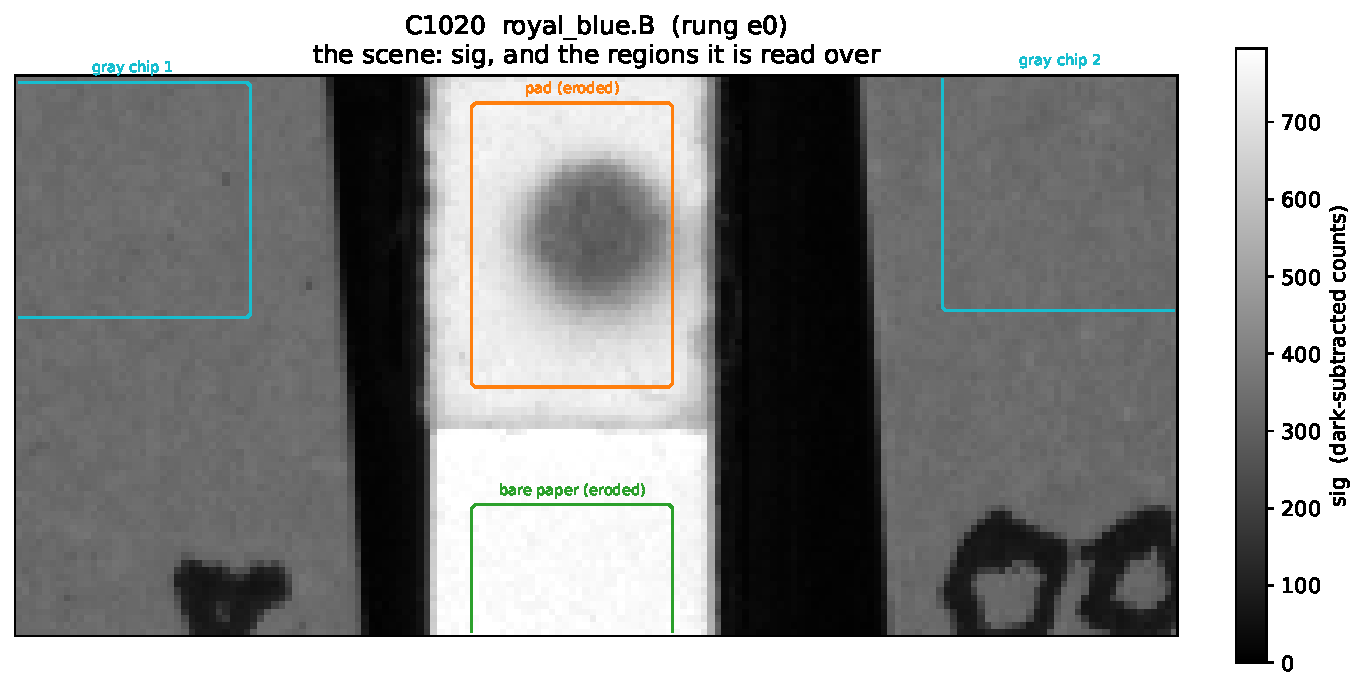
\includegraphics[scale=0.57]{R-inf-guide-C1020-royal-blue.B-1}
	\caption{ %\ref{fig:RinfB1}.  
	The dark-subtracted signal \texttt{sig} for royal\_blue.B on C1020, in
	raw camera counts, cropped to the working area.  Four regions are marked:
	the two gray chips (stage furniture, the reference for $R$), the pad (the
	fitted rectangle, backed off 6 px from its edge), and the strip's own bare
	paper below the pad (the reference for $R_\infty$)).  Chip means here are S1 =
	337.1 and S2 = 334.8 counts; the pad mean is 601.2.  "R against the gray
	chips" means each pad pixel's `sig` will be divided by a reference number
	built from S1 and S2; $R_\infty$ against the bare paper" means that result is
	then divided by the same quantity measured on the paper.
	}
	\label{fig:RinfB1}
\end{figure}

\begin{figure}[h!]
	\centering
	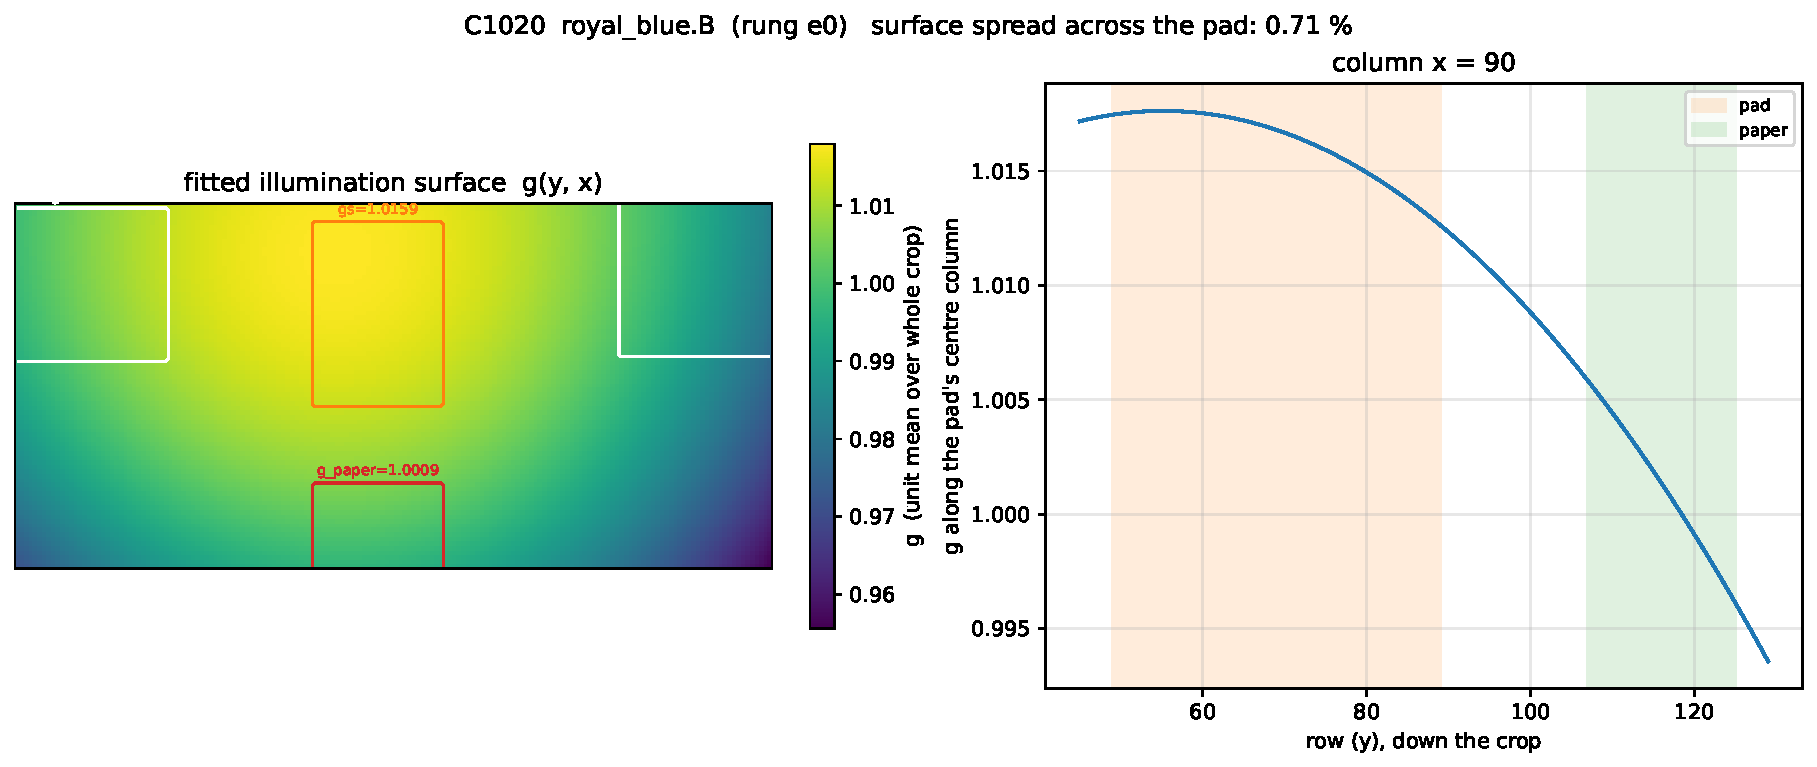
\includegraphics[scale=0.57]{R-inf-guide-C1020-royal-blue.B-2}
	\caption{
	The fitted illumination surface $g(y, x)$ for royal\_blue.B: a
	smooth polynomial (degree 3 down, 1 across), one per cell, scaled so its
	mean over the whole crop is 1.  It is the shape of the lighting with the
	overall level removed.  The anchor weights use only its means over the
	marked regions: g1 = 1.0053, g2 = 0.9921 on the chips, gs = 1.0159 on the
	pad, g\_paper = 1.0009 on the paper.  Right: $g$ along the pad's center
	column.  Across the pad it varies by only 0.71 %; the pad-to-paper step is
	+1.50 % (gs / g_paper = 1.0150).
	}
\label{fig:RinfB2}
\end{figure}

%wrote /home/bill/Projects/Colorimeter/desktop/padanalysis/fig/R_inf_guide_C1020_royal\_blue.B_3.pdf

\begin{figure}[h!]
	\centering
	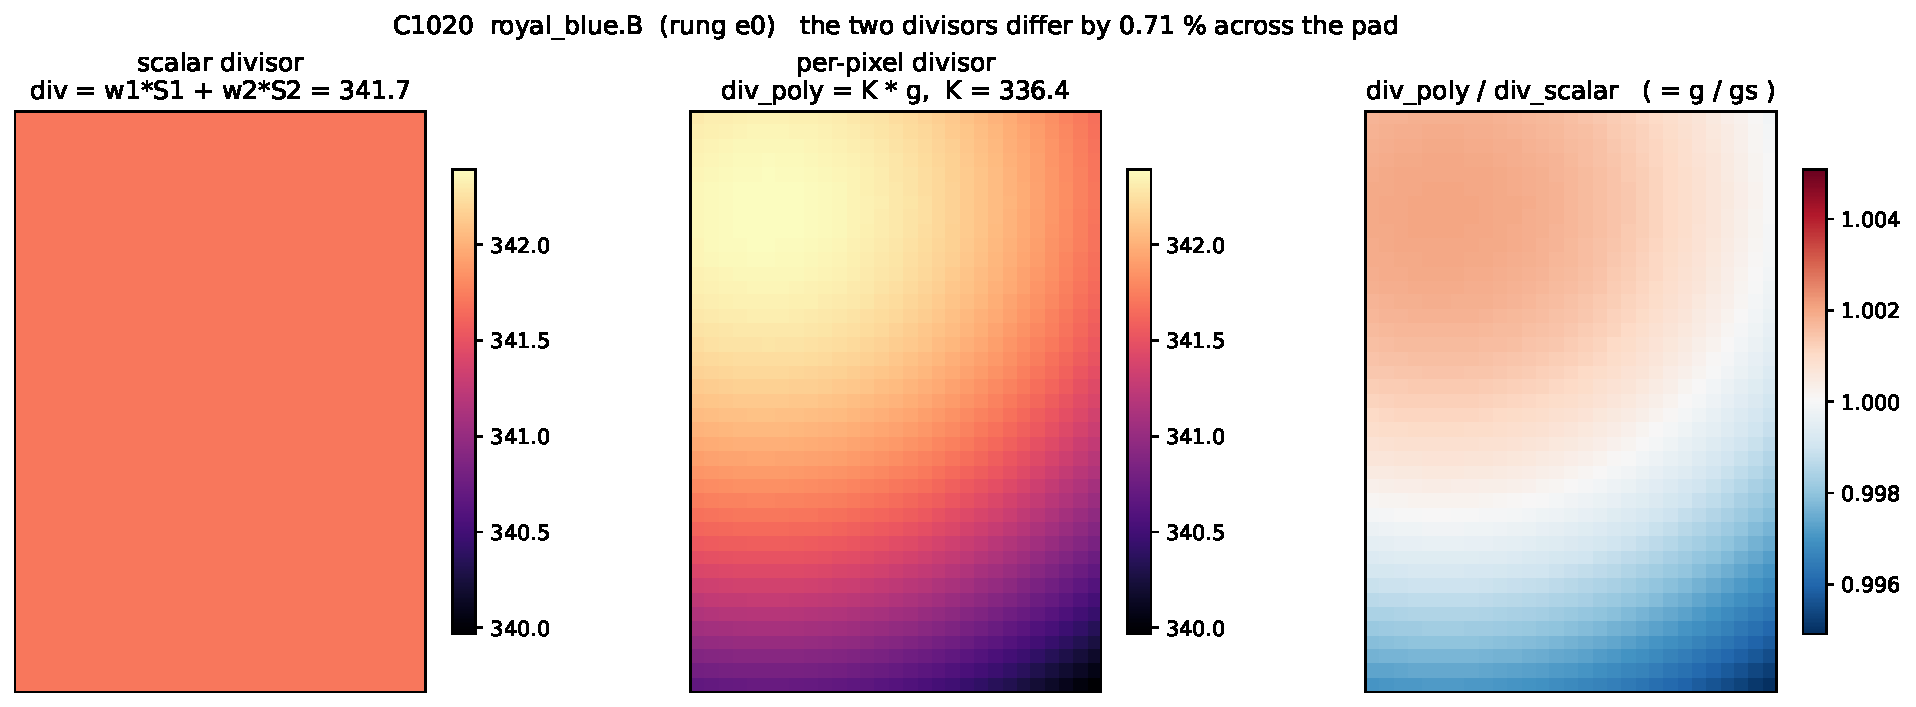
\includegraphics[scale=0.57]{R-inf-guide-C1020-royal-blue.B-3}
	\caption{
	Left: the divisor as `analysis\_1.py` uses it -- one number for
	the whole pad, 341.7 counts, formed from the chip means $S1$, $S2$ and the
	weights $w1 = 0.5317$, $w2 = 0.4852$ (the pad sits a fraction $t = 0.474$ of the
	way from chip 1 to chip 2).  Middle: the per-pixel alternative, 
	$K * g(y, x)$, with $K$ = div\_scalar / gs so the chips still match on average.  Right:
	their ratio, which is exactly g(y, x) / gs -- the surface's variation
	across the pad, 0.71 % peak to peak here.  This is the only thing a per-
	pixel divisor changes about $R$ on the pad.
	}
\label{fig:RinfB3}
\end{figure}

%wrote /home/bill/Projects/Colorimeter/desktop/padanalysis/fig/R_inf_guide_C1020_royal\_blue.B_4.pdf

\begin{figure}[h!]
	\centering
	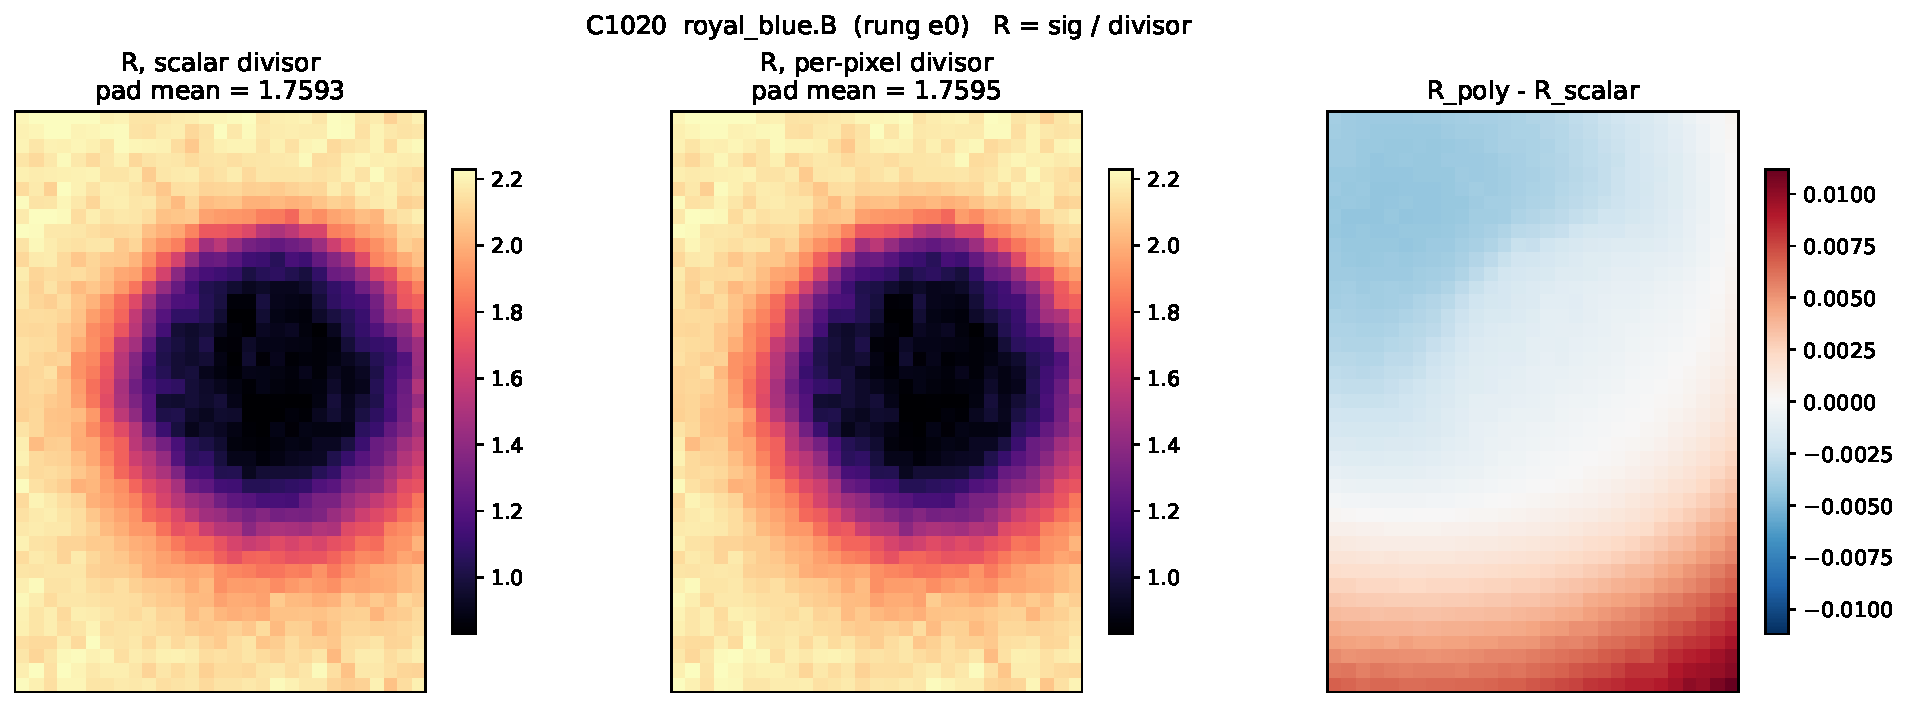
\includegraphics[scale=0.57]{R-inf-guide-C1020-royal-blue.B-4}
	\caption{
	Figure 4.  $R$ for royal\_blue.B, the pad signal divided by the divisor,
	both ways.  The pad-mean values are equal to four decimals (1.7593 vs
	1.7595) -- they must be, because gs is by definition the mean of $g$ over
	the pad, so the two divisors agree on average there.  The per-pixel
	version only removes the gentle across-pad gradient (right panel), max
	0.0112 in $R$ units.  $R = 1$ would mean "as bright as the interpolated
	chips"; bare strip paper runs near 2, a stained pad in a band it absorbs
	runs below 1.
	}
\label{fig:RinfB4}
\end{figure}

	
%wrote /home/bill/Projects/Colorimeter/desktop/padanalysis/fig/R_inf_guide_C1020_royal\_blue.B_5.pdf
	
\begin{figure}[h!]
	\centering
	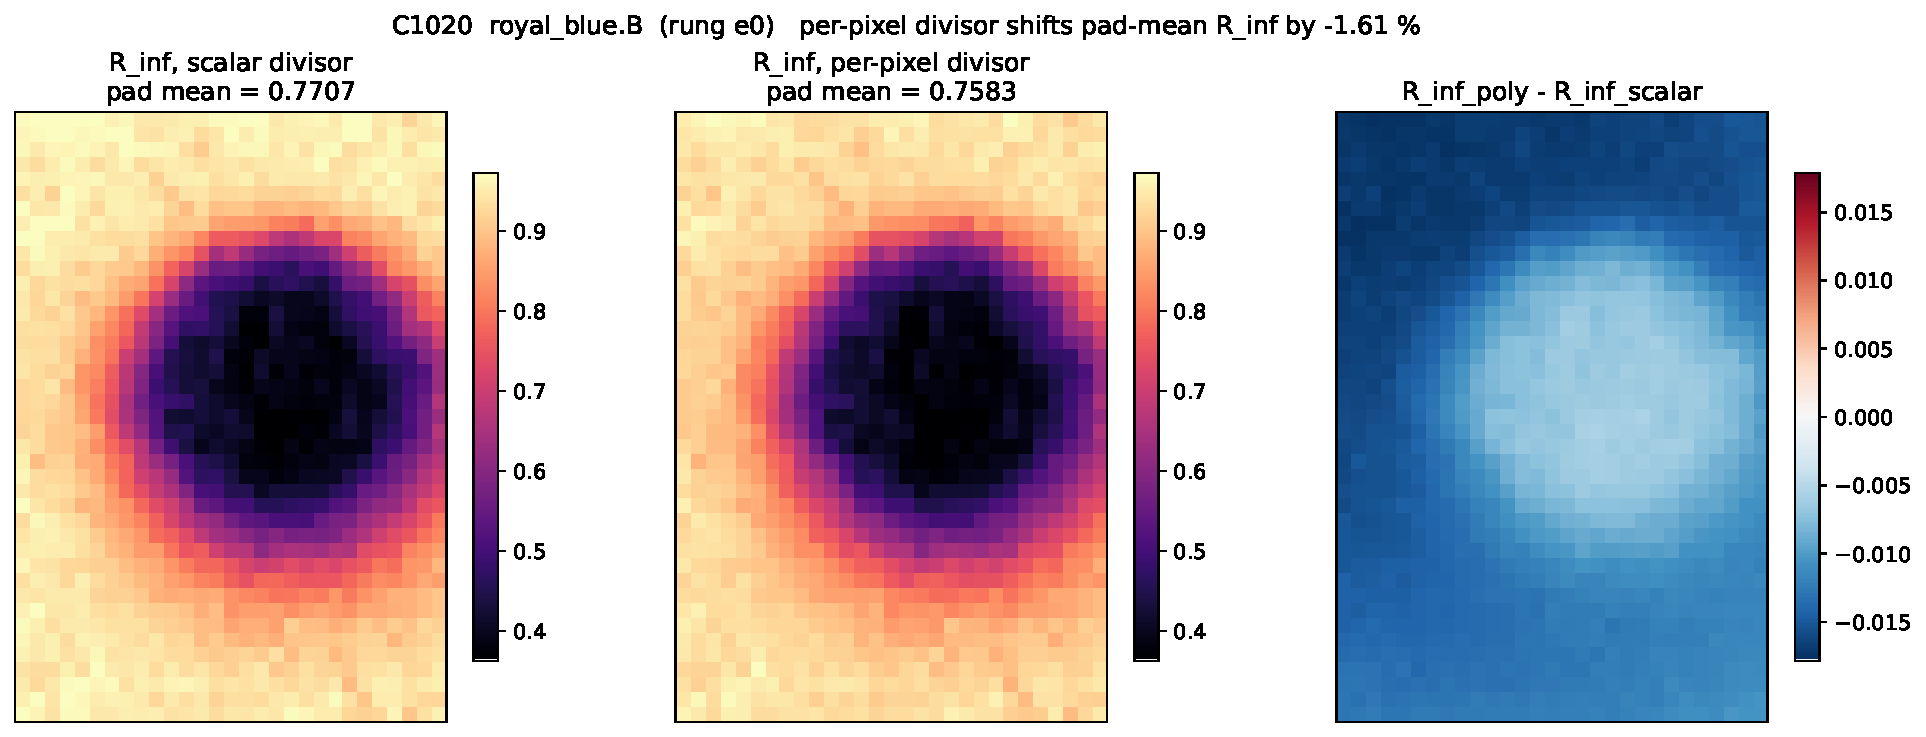
\includegraphics[scale=0.57]{R-inf-guide-C1020-royal-blue.B-5}
	\caption{
	Figure 5.  $R_\infty$ for royal\_blue.B, both ways.  
	With the scalar divisor it cancels: 
	dividing $sig\_pad / div$ by $median(sig\_paper) / div$ leaves
	$sig\_pad / median(sig\_paper)$, with no $div$ in it 
	(checked here: the scalar map matches that div-free form to 1.11e-16).  
	So the scalar divisor's value does not affect $R_\infty$, A or K/S at all.  
	The per-pixel divisor does not cancel 
	-- it divides the pad and the paper each by their own local surface value 
	-- and it moves the pad-mean $R_\infty$ by -1.61\% here.  
	Most of that is the pad-to-paper step in $g$ (+1.50\%), 
	i.e. a modeled estimate of the lighting difference between the two regions, 
	not a sharpening of the map.
	}
\label{fig:RinfB5}
\end{figure}

%wrote /home/bill/Projects/Colorimeter/desktop/padanalysis/fig/R_inf_guide_C1020_royal\_blue.B_6.pdf
\clearpage	
\begin{figure}[h!]
	\centering
	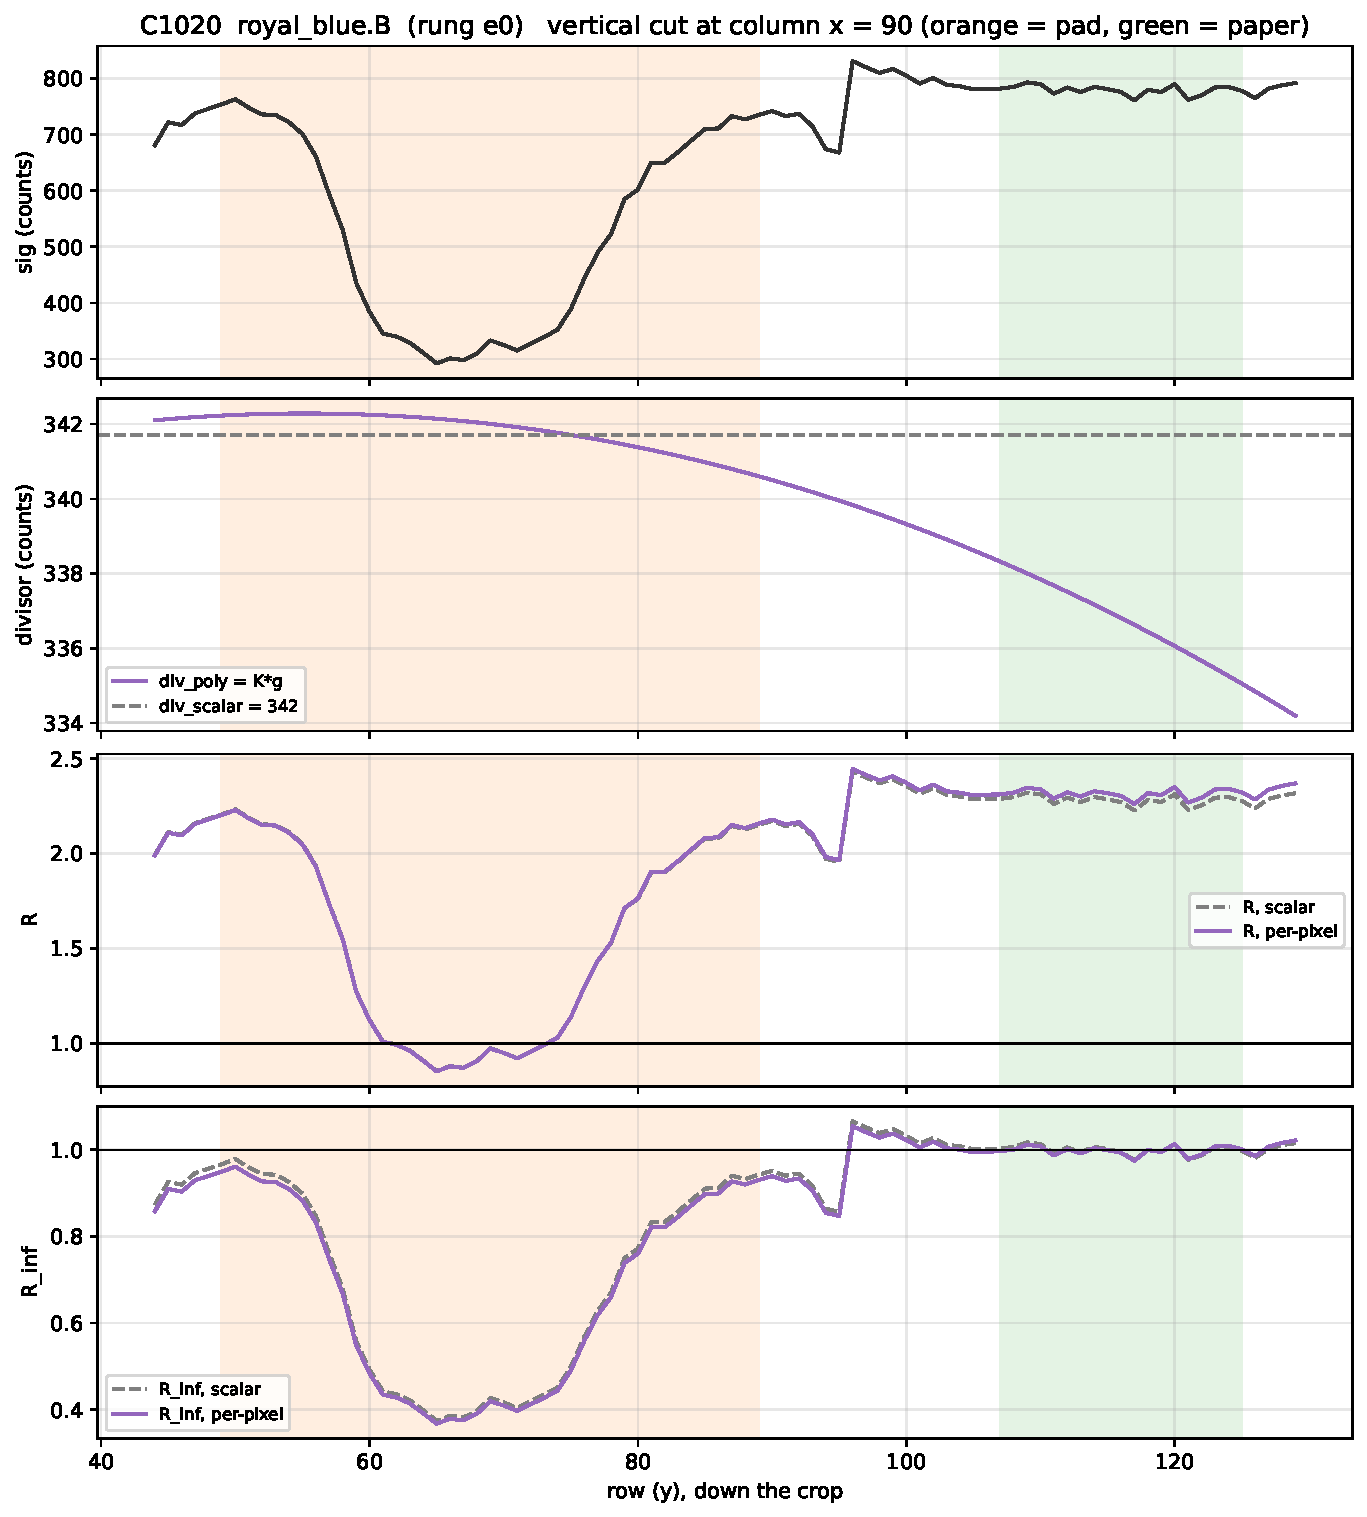
\includegraphics[scale=0.57]{R-inf-guide-C1020-royal-blue.B-6}
	\caption{
	Figure 6.  A single column of pixels through the pad center (x = 90) and
	on down into the paper region, royal\_blue.B on C1020.  Top to bottom: the
	raw signal; the two divisors (the scalar is a flat line, the polynomial a
	gentle curve of the same K * g); $R$ each way; $R_\infty$ each way.  The pad
	band and the paper band are shaded.  On $R_\infty$ the two curves are near-
	parallel inside the pad -- the per-pixel divisor is not reshaping the pad
	profile -- but they are offset, because the polynomial applied a different
	correction over the pad than over the paper.
	}
\label{fig:RinfB6}
\end{figure}

\clearpage	
\begin{figure}[h!]
	\centering
	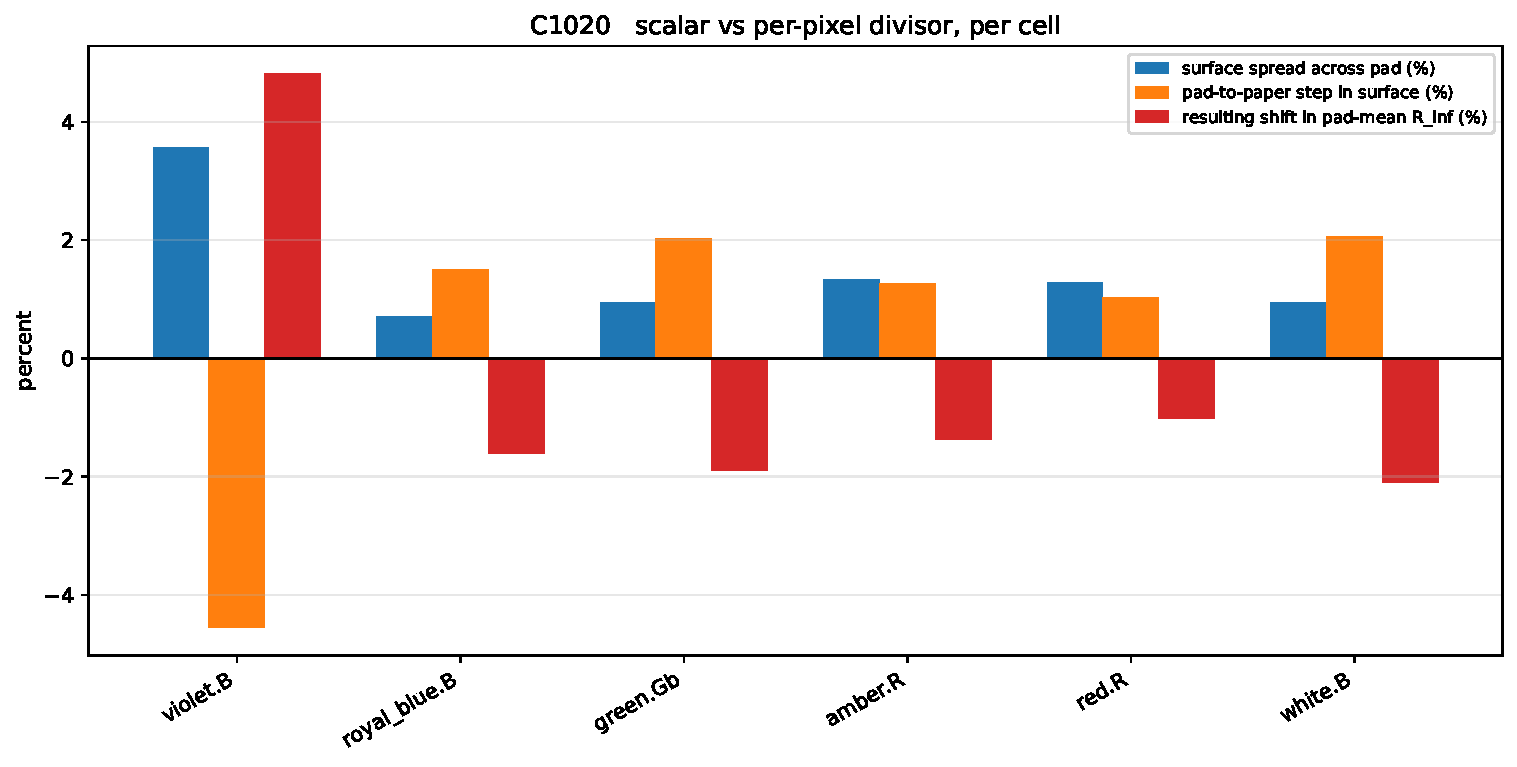
\includegraphics[scale=0.57]{R-inf-guide-C1020-survey}
	\caption{
	The same comparison across 6 cells of C1020.  Blue: how much
	the fitted surface varies across the pad (what a per-pixel divisor removes
	from the map).  Orange: the surface's pad-to-paper step (the modelled
	lighting difference between the two regions).  Red: the net shift a per-
	pixel divisor puts on the pad-mean$R_\infty$.  The shift is cell-dependent and
	changes sign -- short-wavelength cells like violet.B move one way, the
	rest the other -- so adopting it would change the shape of the pad
	spectrum, not just its level.  violet.B is also the lowest-signal, most-
	vignetted cell, where the low-order surface fit is least certain.
	}
\label{fig:Rinfsurvey}
\end{figure}

\begin{table}[h]
	\centering
	\caption{Scalar vs per-pixel divisor}
	\begin{tabular}{lccccc}
		\toprule
		cell & pad grad\% & pad/paper\% & $R_\infty$ scalar & $R_\infty$ poly & shift\%\\
		\midrule
		violet.B     & 3.56 &-4.55 & 0.6595 & 0.6913 &  4.81 \\
		royal\_blue.B & 0.71 & 1.50 & 0.7707 & 0.7583 & -1.61 \\
		blue.B       & !   &  !    &   !    &   !    &  !    \\
		green.Gb     & 0.94 & 2.03 & 0.9934 & 0.9745 & -1.90 \\
		amber.R      & 1.33 & 1.27 & 1.0512 & 1.0367 & -1.38 \\
		red.R        & 1.28 & 1.04 & 1.0381 & 1.0276 & -1.01 \\
		white.B      & 0.95 & 2.07 & 0.8384 & 0.8208 & -2.10 \\
		\bottomrule
	\end{tabular}
\end{table}
 
\subsection{conclusions} 

Claude concludes: 

Bottom line.  $R_\infty$, $A$ and $K/S$ do not see the scalar divisor -- it
cancels.  
A per-pixel polynomial divisor would change $R_\infty$, but mostly by
importing the fitted surface's estimate of the lighting difference between
the pad and the paper (+1.50 \% for this cell), which is a claim about the
flat-field model rather than a finer measurement.  The across-pad gradient
it also removes is 0.71 \%.  Keep the scalar divisor for $R_\infty$.  If the
pad-to-paper offset is worth correcting, test it on its own -- photograph
one blank strip with the pad slid down to the paper's position and measure
the ratio directly -- rather than trusting the low-order surface to supply
it, especially for the short-wavelength cells where it and the survey
disagree most.

But I disagree. 


\clearpage
\newpage
%======================================================================
\section{Reference documents}
%======================================================================

\begin{longtable}{@{}L{5.7cm}L{9.7cm}@{}}
\toprule
\textbf{Document} & \textbf{What it covers} \\
\midrule
\file{desktop/padanalysis/padphot.py} & Module docstring: the whole chain and
the three traps (K and S do not separate; $f(R)$ is scale-sensitive; $A$ and
$f(R)$ are different transforms).  Per-function docstrings carry each
formula. \\
\file{desktop/padanalysis/HOWTO.md} & \S\,8.2--8.4 (lines 388--467): the ROI
names, the one-function-per-step table (\Rinf{} row at line 421), and the
arithmetic check (``\code{R\_inf} must be 1.0000'', line 460). \\
\file{tex/gutzeit\_analysis.tex} & \S\,``Reflectance photometry'' (lines
894--931): Kubelka--Munk, equation \code{eq:km} for $f(\Rinf)$, the four
assumptions including (iv) ``\Rinf{} measured relative to a stable diffuse
white'', and \code{eq:dks} for the blank subtraction. \\
\file{desktop/padanalysis/chemistry.py} & The \code{Reduction} class: the
same quantity as \code{rho}, built from \code{records.json} rather than the
per-cell balanced pipeline. \\
\bottomrule
\end{longtable}

\end{document}
